\documentclass[manuscript, letterpaper]{aastex6}

% to-do list
% ----------

% style notes
% -----------
% - This file generates by Makefile; don't be typing ``pdflatex'' or some bullshit.
% - Line break between sentences to make the git diffs readable.
% - Use \, as a multiply operator.
% - Reserve () for function arguments; use [] or {} for outer shit.
% - Use \sectionname not Section, \figname not Figure, \documentname not Article or Paper or paper.

\include{gitstuff}
% ----------------------------------- %
% start of AASTeX mods by DWH and DFM %
% ----------------------------------- %

\setlength{\voffset}{0in}
\setlength{\hoffset}{0in}
\setlength{\textwidth}{6in}
\setlength{\textheight}{9in}
\setlength{\headheight}{0ex}
\setlength{\headsep}{\baselinestretch\baselineskip} % this is 2 lines in ``manuscript''
\setlength{\footnotesep}{0in}
\setlength{\topmargin}{-\headsep}
\setlength{\oddsidemargin}{0.25in}
\setlength{\evensidemargin}{0.25in}

\linespread{0.54} % close to 10/13 spacing in ``manuscript''
\setlength{\parindent}{0.54\baselineskip}
\hypersetup{colorlinks = false}
\makeatletter % you know you are living your life wrong when you need to do this
\long\def\frontmatter@title@above{
\vspace*{-\headsep}\vspace*{\headheight}
\noindent\footnotesize
{\noindent\footnotesize\textsc{\@journalinfo}}\par
{\noindent\scriptsize Preprint typeset using \LaTeX\ style AASTeX6
with modifications by DWH and DFM.
}\par\vspace*{-\baselineskip}\vspace*{0.625in}
}%
\long\def\frontmatter@abstractheading{%
\makeaffils
  \vspace*{-\baselineskip}\vspace*{1.5pt}
  \vspace*{0.13189in}
 \begingroup
  \centering
  \abstractname
  \vskip 1mm
  \par
 \endgroup
 \everypar{\rightskip=0.0in\leftskip=\rightskip}\par
}%
\def\frontmatter@keys@format{\vspace*{0.5mm}%
  \settowidth{\keys@width}{\normalsize\@keys@name}%
  \rightskip=0.0in\leftskip=\rightskip\parindent=0pt%
    \hangindent=\keys@width\hangafter=1\normalsize\raggedright}%
\def\twodigits#1{\ifnum#1<10 0\fi\the#1}
\def\mydate{\leavevmode\hbox{\the\year-\twodigits\month-\twodigits\day}}
\makeatother
\renewcommand{\today}{\mydate}

% Section spacing:
\makeatletter
\let\origsection\section
\renewcommand\section{\@ifstar{\starsection}{\nostarsection}}
\newcommand\nostarsection[1]{\sectionprelude\origsection{#1}}
\newcommand\starsection[1]{\sectionprelude\origsection*{#1}}
\newcommand\sectionprelude{\vspace{1em}}
\let\origsubsection\subsection
\renewcommand\subsection{\@ifstar{\starsubsection}{\nostarsubsection}}
\newcommand\nostarsubsection[1]{\subsectionprelude\origsubsection{#1}}
\newcommand\starsubsection[1]{\subsectionprelude\origsubsection*{#1}}
\newcommand\subsectionprelude{\vspace{1em}}
\makeatother

\widowpenalty=10000
\clubpenalty=10000

\sloppy\sloppypar

% ------------------ %
% end of AASTeX mods %
% ------------------ %


% packages
\definecolor{cbblue}{HTML}{3182bd}
\usepackage{microtype}  % ALWAYS!
\usepackage{amsmath}
\hypersetup{backref,breaklinks,colorlinks,urlcolor=cbblue,linkcolor=cbblue,citecolor=black}

% define macros for text
\newcommand{\project}[1]{\textsl{#1}}
\newcommand{\acronym}[1]{{\small{#1}}}
\newcommand{\gaia}{\project{Gaia}}
\newcommand{\rave}{\project{\acronym{RAVE}}}
\newcommand{\apogee}{\project{\acronym{APOGEE}}}
\newcommand{\documentname}{\textsl{Article}}
\newcommand{\sectionname}{Section}
\newcommand{\figname}{Figure}
\newcommand{\eqname}{Equation}
\newcommand{\dr}{\acronym{DR1}}

% define macros for math
\newcommand{\given}{\,|\,}
\newcommand{\normal}{{\mathcal{N}}}
\newcommand{\dd}{\mathrm{d}}
\newcommand{\transp}[1]{{#1}^{\!\mathsf{T}}}
\newcommand{\inv}[1]{{#1}^{-1}}
\newcommand{\bs}[1]{\boldsymbol{#1}}
\newcommand{\vperp}{\bs{v}^\perp}
\newcommand{\propm}{\bs{\mu}}
\newcommand{\matrx}[1]{\mathbf{#1}}
\newcommand{\kms}{\rm km~s^{-1}}
\newcommand{\data}{\mathrm{data}}
\newcommand{\snr}{[S/N]_\varpi}

% TODO
\newcommand{\todo}[1]{{\color{red}TODO: #1}}

\begin{document}\sloppy\sloppypar\raggedbottom\frenchspacing % trust me

\title{Co-moving stars in \textsl{Gaia DR1}}
\author{Adrian M. Price-Whelan\altaffilmark{\pu,\adrn},
        Semyeong Oh\altaffilmark{\pu},
        David W. Hogg\altaffilmark{\ccpp,\mpia},
        Timothy D. Morton\altaffilmark{\pu},
        David N. Spergel\altaffilmark{\pu,\cca}
}

% Affiliations
\newcommand{\pu}{1}
\newcommand{\adrn}{2}
\newcommand{\ccpp}{3}
\newcommand{\mpia}{4}
\newcommand{\cca}{5}

\altaffiltext{\pu}{Department of Astrophysical Sciences,
                   Princeton University, Princeton, NJ 08544, USA}
\altaffiltext{\adrn}{To whom correspondence should be addressed:
                     \texttt{adrn@princeton.edu}}
\altaffiltext{\ccpp}{Center for Cosmology and Particle Physics,
                     Department of Physics,
                     New York University, 4 Washington Place,
                     New York, NY 10003, USA}
\altaffiltext{\mpia}{Max-Planck-Institut f\"ur Astronomie,
                     K\"onigstuhl 17, D-69117 Heidelberg, Germany}
\altaffiltext{\cca}{Simons Center for Computational Astrophysics, ...,
                    New York, NY XXXXX, USA}

\begin{abstract}
% Context
The primary sample of the \gaia\ \textsl{First Data Release} is the brand-new
\textsl{Tycho-Gaia Astrometric Solution}. The precision and size of this sample
creates an opportunity to find new binary stars and moving groups, especially
rare binaries or sparsely populated groups.
% Aims
Here we seize this opportunity.
% Methods
We use a justified marginalized likelihood ratio test to separate
pairs of stars with surprisingly similar three-space velocities from
those consistent with being drawn independently from the field
population.  Although we perform some visualizations using a
(bias-corrected) inverse parallax as a distance, the likelihood test
works in the observable space and uses the \gaia\ noise model
responsibly.
% Results
We find pairs of comoving stars out to very wide
separations, including separations of a few parsecs! There does not
seem to be any tidal-disruption feature in the separation distribution
at sub-parsec scales. Pairs at separations beyond a
parsec---whether they are bound in a multiple system or drifting
apart---must be very short-lived. The photometric properties of the
members of these pairs are consistent with youth. The prospects for
testing stellar models and chemical abundance measurements are
superficially discussed.
\end{abstract}

\keywords{
  binaries: visual
  ---
  methods: statistical
  ---
  open clusters and associations: general
  ---
  parallaxes
  ---
  proper motions
  ---
  stars: formation
}

\section{Introduction} \label{sec:intro}

Two stars moving with similar full-space velocity vectors (``co-moving stars'')
are either members of a widely-separated stellar multiplet, or remnants of a
dispersing stellar system.

Widely-separated binary stars are weakly bound binary star systems with
semi-major axes larger than $a \gtrsim 10^{-3}~{\rm pc}$. It is generally
assumed that the stars in a wide binary form from gas with the same chemical
composition and are separated enough that there is no interaction or minimal
cross-pollution as the more massive star evolves (\citealt{todo}). Because the
binding energy of these systems is so low, if wide binary stars survive for many
Gigayears their existence alone places limits on the tidal field of the Galaxy
(\citealt{todo}) and the graininess of the gravitational field (\citealt{todo}).
In this picture, a remaining puzzle is how these systems survive the dense
stellar environments of the birth clusters in which they form. Wide binaries are
therefore important tools for studying small-scale star formation and the
large-scale Galactic mass distribution. These stars will appear to be co-moving
with velocity differences comparable to the binary orbital velocity at the
given separation.

At the largest separations, $a \gtrsim 1~{\rm pc}$, co-moving stars are likely
either remnants of disrupting stellar systems or young wide binary stars: at
these extreme separations, the Galactic tidal field would disrupt binary stars
within $t_{\rm disrupt} \lesssim XX~{\rm Gyr}$. Unbound open clusters with
velocity dispersions $\sigma_v \lesssim 1~\kms$ in the Galactic disk disrupt
quickly leaving small streams of stars with the same chemical abundances
(\citealt{chemicaltaggingstuff}). Disrupting or disrupted globular clusters and
dwarf galaxies also produce streams of stars with similar chemical properties
but with larger velocity differences (\citealt{streampeeps}). Stars from such
systems at similar orbital phases will appear to be co-moving with velocity
differences comparable to the internal velocity dispersions, $\sigma_v \approx
1$--$10~\kms$.

To date, thousands of candidate co-moving star pairs have been identified by
searching for stars with common proper motions (\citealt{Luyten:1979,
Poveda:1994, Allen:2000, Gould:2003, Chaname:2004, Lepine:2007,
Alonso-Floriano:2015}). \todo{how is our search different? (1) we have distance, (2) bigger volume than Hipparcos, (3) we use the data properly, (4) we don't cut on distance or on magnitude of proper motion -- we cut on parallax S/N}
% Cite:
% Tokovinin & Lepine 2012
% https://ui.adsabs.harvard.edu/#abs/2012ApJ...757..170A/abstract
% https://ui.adsabs.harvard.edu/#abs/2012AJ....144..102T/abstract
% https://ui.adsabs.harvard.edu/#abs/2014ApJ...790..158A/abstract

% Many searches find things close in angular separation, but need pms / distance

% Two stars moving with full-space velocity vector differences $\lesssim 1~\kms$
% with orbital semi-major axes $a \gtrsim 10^-3~{\rm pc}$.

Useful for:
- star cluster disruption and dispersal
- chemical abundance comparison (no interaction)
- dynamics

In either case, co-moving stars are of great interest
for studying the destruction of star clusters and dwarf galaxies, the tidal
field and small-scale properties of the mass distribution in the Milky Way, and
chemical uniformity and star formation processes.

\section{Data} \label{sec:data}

The primary data set used in this \documentname\ is the Tycho-Gaia Astrometric
Solution (TGAS), released as a part of Data Release 1 of the Gaia mission
(\citealt{many}). TGAS contains astrometric measurements (sky position,
parallax, and proper motions) and associated covariance matrices for a large
fraction of the \project{Tycho-2} catalog (\citealt{tycho2}) with median
astrometric precision equivalent to the \project{Hipparcos} catalog ($\approx
0.3~{\rm mas}$; \citealt{hipparcos}). In terms of parallax signal-to-noise
($\snr = \varpi/\sigma_\varpi$), the TGAS catalog contains 1240114 stars with
$\snr > 4$, 619618 stars with $\snr > 8$, and 197105 stars with $\snr > 16$. The
increase in precision over Tycho-2 and increase in volume over Hipparcos makes
the TGAS catalog a powerful data set to search for widely-separated, co-moving
stars.

In the sections that follow, we construct a statistical model that propagates
the non-trivial uncertainties in the data to our beliefs about the likelihood
that a given pair are co-moving. Here, we instead compute quantities directly
from the astrometric measurements to visualize and emphasize the quality of the
data. For each star with $\snr > 16$, we use the reported parallax and parallax
error to compute a distance corrected for the Lutz-Kelker bias
(\citealt{lutzkelker}):
\begin{equation}
  d_{\rm LK} = 1000 \, \left[\frac{\varpi}{2} \,
    \left(1 + \sqrt{1 - \frac{16}{\snr^2}} \right) \right]^{-1} \, {\rm pc}
\end{equation}
We use this distance and the sky positions of each source to compute 3D
Cartesian positions, $\boldsymbol{x}$, for all stars and find the nearest
neighbor to each source in 3-space using the KDTree implementation in
\project{scikit-learn} (\citealt{scikit-learn}). We remove duplicates from
this sample and are left with 138962 pairs of stars. For all pairs, we then
compute the tangential velocity difference
\begin{equation}
  |\Delta \bs{v}_{\rm t}| = d_{\rm LK} \,
                            \sqrt{(\mu_{\alpha,1}-\mu_{\alpha,2})^2 +
                                  (\mu_{\delta,1}-\mu_{\delta,2})^2}
\end{equation}
\figname~\ref{fig:dv-sep} shows these quantities plotted for all pairs that pass
the above signal-to-noise cut. Pairs with small physical separation also tend to
have small velocity differences. Intriguingly, there appear to be an abundance
of pairs with small velocity separation at separations $|\delta\bs{x}| \gtrsim
1~{\rm pc}$.

\begin{figure*}[p]
\begin{center}
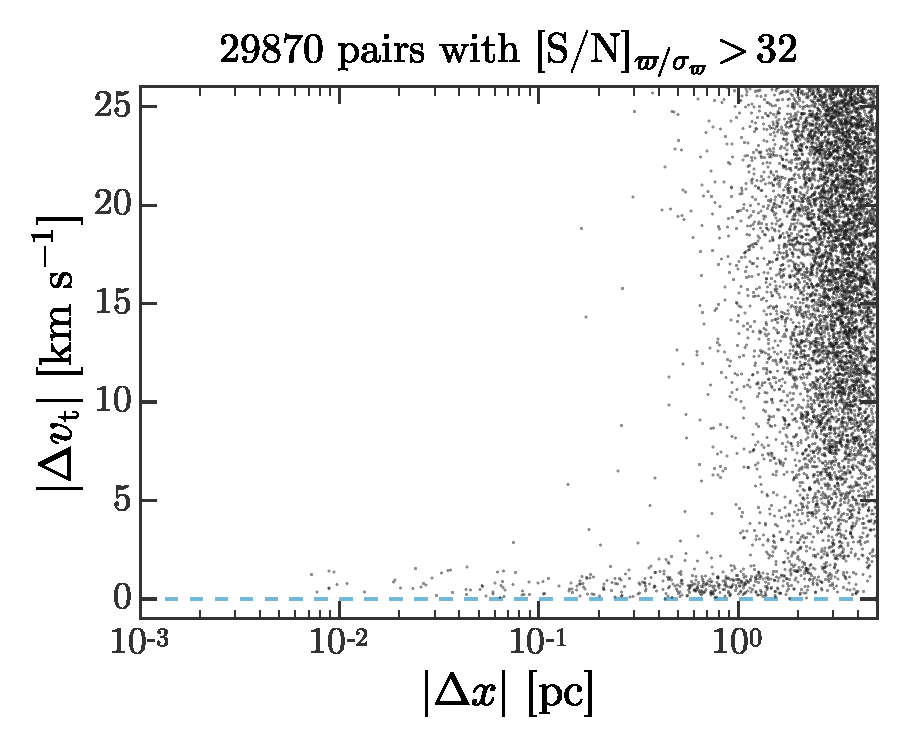
\includegraphics[width=\textwidth]{figures/dv-sep.pdf}
\end{center}
\caption{%
Difference in tangential velocity vs. physical separation for pairs of stars
selected to be nearest neighbors in separation. Dashed line shows zero velocity
difference. Note the points with small velocity difference: these are likely
widely-separated binary stars.
\label{fig:dv-sep}}
\end{figure*}

\todo{More naive visualizations, or save for the full sample?}

\section{Methods} \label{sec:methods}

For a given pair of stars $(i,j)$, we compute the fully marginalized likelihood
(FML) that the pair has the same 3-space velocity (hypothesis 1,
$\mathcal{L}_1$) and the FML of the stars having different 3-space velocities
(hypothesis 2, $\mathcal{L}_2$). We use the ratio of these FMLs as a scalar for
selecting candidate widely-separated binary stars. \gaia\ \dr\ only contains
parallax, $\varpi$, and two proper motion components, $\propm = (\mu_\alpha,
\mu_\delta)$ for each star, so for the majority of sources we only have
information about the tangential velocities of the stars. Where there is overlap
with \rave\ or \apogee, some number of observed radial velocities, $v_r$, with
observed variances $\sigma^2_{v_r}$ (independent of the \gaia\ data) may also be
available. We assume that the uncertainties in these observed quantites are
known with covariance matrix $\matrx{C}$. The likelihood functions $L_1, L_2$
are marginalized over true 3-space velocity and distance for each star in the
pair.
\begin{align}
  \mathcal{L}_1 &=
    \int \, \dd d_i \, \dd d_j \, \dd^3 \bs{v} \,
    L_i(\bs{v}, d_i) \,
    L_j(\bs{v}, d_j) \,
    p(\bs{v}) \, p(d_i \given \varpi_i) \, p(d_j \given \varpi_j) \\
  \mathcal{L}_2 &=
    \int \, \dd d_i \, \dd d_j \, \dd^3 \bs{v}_i \, \dd^3 \bs{v}_j \,
    L_i(\bs{v}_i, d_i) \,
    L_j(\bs{v}_j, d_j) \,
    p(\bs{v}_i) \, p(\bs{v}_j) \, p(d_i \given \varpi_i) \, p(d_j \given \varpi_j) \label{eq:hyp2}
\end{align}
where
\begin{align}
  L(\bs{v}, d) &=
    \left[\det\left(\frac{\matrx{C}^{-1}}{2\pi}\right)\right]^{1/2} \,
    \exp \left[ -\frac{1}{2} \transp{\left(\bs{x} - \bs{x}_\theta \right)} \,
    \matrx{C}^{-1} \,
    \left(\bs{x} - \bs{x}_\theta \right) \right] \\
  \bs{x} &= \transp{(\begin{array}{c c c} \mu_\alpha &
    \mu_\delta & v_r \end{array})} \\
  \bs{x}_\theta &= \transp{\left(\begin{array}{c c c} d^{-1}\,v_\alpha &
    d^{-1}\,v_\delta & \tilde{v}_r \end{array}\right)}
\end{align}
and we compute the posterior pdfs for the true distances, $p(d\given\varpi)$,
using a uniform space density prior \citep{Astraatmadja:2016} on heliocentric
distance
\begin{equation}
  p(d) \propto d^2
\end{equation}
We assume Gaussian priors on the true velocity components
\begin{equation}
  p(\bs{v}) = \normal(0,25)~\kms
\end{equation}

For hypothesis 1, the integral over velocity is non-trivial because the same
``true'' 3-space velocity vector projects into tangential velocity components
differently depending on sky position ($v_\alpha = v_\alpha(\bs{v}, \alpha,
\delta)$). The marginalization integral for hypothesis 2 is simpler because the
integral in \eqname~\ref{eq:hyp2} can be split into the product of two simpler
integrals $\mathcal{L}_2 = Q_i \, Q_j$ where
\begin{equation}
  Q = \int \, \dd d \, \dd^3 \bs{v} \, L(\bs{v}, d) \, p(\bs{v}) \, p(d\given\varpi)
\end{equation}
In either case, the marginalization over true 3-space velocity can be performed
analytically; we derive the relevant expressions in
\sectionname~\ref{sec:appendix}. After marginalizing over velocity, the
likelihood integrands only depend on distance; we numerically compute the
integrals over the true distances to each star in a pair, $d_1,d_2$, using Monte
Carlo integration with $K$ samples from the distance posterior pdfs:
\begin{equation}
  \int \, \dd d \, \tilde{L}(d) \, p(d\given\varpi) \approx
    \frac{1}{K} \, \sum_k^K \, \tilde{L}(d_k)
\end{equation}
Through experimentation, we have found that $K=128$ samples are sufficient for
estimating the above integrals for stars with a wide range in parallax
signal-to-noise.

\section{Results 1: A catalog of candidate wide binaries}

\todo{Galactic context / orbits}

\section{Results 2: Star clusters and cluster remnants}

\section{Conclusions}

\acknowledgements

This research was partially supported by the \acronym{NSF} (grants
  \acronym{IIS-1124794}, \acronym{AST-1312863}, \acronym{AST-1517237}),
  \acronym{NASA} (grant \acronym{NNX12AI50G}),
  and the Moore-Sloan Data Science Environment at \acronym{NYU}. The data
analysis presented in this article was partially performed on computational
resources supported by the Princeton Institute for Computational Science and
Engineering (PICSciE) and the Office of Information Technology's High
Performance Computing Center and Visualization Laboratory at Princeton
University.

\software{The code used in this project is available from
\url{https://github.com/smoh/gaia-wide-binaries} under the MIT open-source
software license. This version was generated at git commit
\texttt{\githash\,(\gitdate)}.
This research additionally utilized:
    \texttt{Astropy} (\citealt{Astropy-Collaboration:2013}),
    %\texttt{emcee} (\citealt{Foreman-Mackey:2013}),
    \texttt{IPython} (\citealt{Perez:2007}),
    \texttt{matplotlib} (\citealt{Hunter:2007}),
    and \texttt{numpy} (\citealt{Van-der-Walt:2011}).}

% \facility{\sdssiii, \apogee}

\bibliographystyle{aasjournal}
\bibliography{refs}

\appendix

\section{Some mathematics relevant to the above} \label{sec:appendix}

\todo{clean this up}

In what follows, all vectors are column vectors, unless we have transposed them.
We indicate whether a symbol represents a scalar, vector, or tensor
(matrix) by context, not typesetting.
Properties of the squared exponential:
\begin{eqnarray}
  \ln\left[\int\exp(-\frac{1}{2}\,\transp{[x-\nu]}\,\inv{A}\,[x-\nu] - \Delta)\,\dd x\right]
  &=& +\frac{1}{2}\ln ||2\pi\,A|| -\Delta
  \quad ,
\end{eqnarray}
where $x$ and $\nu$ are $D$-dimensional vectors, $A$ is a positive definite
matrix, $\Delta$ is a scalar, and the integral is implicitly over all
of $D$-dimensional $x$-space.
We will need to complete squares.
If we equate
\begin{eqnarray}
  \frac{1}{2}\,\transp{[x-\nu]}\,\inv{A}\,[x-\nu] + \Delta
  &=& \frac{1}{2}\,\transp{x}\,\inv{A}\,x + \transp{x}\,B\,b + C
  \quad ,
\end{eqnarray}
where $B\,b$ is a $d$-vector, and $C$ is a scalar, then we find
\begin{eqnarray}
  \nu &=& -A\,B\,b
  \\
  \Delta & = & C - \frac{1}{2}\,\transp{\nu}\,\inv{A}\,\nu
  \quad .
\end{eqnarray}

Now in this case, we want to write down the probability density for the data
given the distances and velocity (the likelihood), and the prior pdf for
the velocity, and their product.
The prior pdf for the velocity is Gaussian:
\begin{eqnarray}
  p(v) &=& \normal(v\given 0,V)
  \\
  \ln p(v) &=& -\frac{1}{2}\,\ln||2\pi\,V|| -\frac{1}{2}\,\transp{v}\,\inv{V}\,v
  \\
  V &=& \sigma_v^2\,I
  \quad ,
\end{eqnarray}
where $v$ is the three-vector velocity, and $V$ is an isotropic
variance tensor.
Similarly, the likelihood for the data is also a Gaussian.
Before we write that down, we will make some definitions.
We construct a velocity-space data vector $y$ as follows:
\begin{eqnarray}
  \transp{y} &\equiv& [(d_1\,\mu_{\alpha1}), (d_1\,\mu_{\delta1}),
                       (d_2\,\mu_{\alpha2}), (d_2\,\mu_{\delta2})] \quad \mbox{or}
  \\
  \transp{y} &\equiv& [(d_1\,\mu_{\alpha1}), (d_1\,\mu_{\delta1}), (v_{r1}),
                       (d_2\,\mu_{\alpha2}), (d_2\,\mu_{\delta2}), (v_{r2})]
  \quad ,
\end{eqnarray}
where we have given two versions, a 4-component and an 6-component
version (depending on whether there are measured radial velocities),
the subscripts 1, 2 refer to the first and second stars (arbitrarily
ordered) of the pair, we have multiplied the strict observables by
distances $d_1, d_2$, which we are permitted to do (because we are
\emph{conditioning} on $d_1, d_2$), and note the wacky minus-ones.
The vector $y$ is a column vector that we have transposed to make it
easy to write down.
Fundamentally, our H1 model (same velocity) is
\begin{eqnarray}
  y &=& M\,v + \mathrm{noise}
  \\
  \transp{M} &=& [\hat{\alpha_1}, \hat{\delta_1},
                  \hat{\alpha_2}, \hat{\delta_2}] \quad \mbox{or}
  \\
  \transp{M} &=& [\hat{\alpha}_1, \hat{\delta}_2, \hat{r}_1,
                  \hat{\alpha}_2, \hat{\delta}_2, \hat{r}_2]
  \quad,
\end{eqnarray}
where $M$ is a $6\times 3$ or $8\times 3$ design matrix, with zeros
in two rows, and unit vectors along the other rows.
The noise (in the $y$ vector) is drawn from a Gaussian with ($6\times 6$ or $8\times 8$)
covariance matrix $\Sigma$, constructed from the distances $d_1, d_2$ and
the \gaia-provided individual-object covariance matrices.
Given all these definitions, the likelihood function is
\begin{eqnarray}
  p(\data\given v,d_1,d_2) &=& d_1^2\,d_2^2\,\normal(y\given M\,v, \Sigma)
  \\
  \ln p(\data\given v,d_1,d_2) &=& 3\,\ln d_1 + 3\,\ln d_2
  -\frac{1}{2}\,\ln||2\pi\,\Sigma|| \nonumber \\ && \quad
  -\frac{1}{2}\,\transp{[y-M\,v]}\,\inv{\Sigma}\,[y-M\,v]
  \quad ,
\end{eqnarray}
where the factor of $d_1^2\,d_2^2$ converts to units of per \gaia\ data
from units of per $y$.

Now we multiply together (add in the log) and complete the square.
We get, in the original parameterization:
\begin{eqnarray}
  \inv{A} &=& [\transp{M}\,\inv{\Sigma}\,M+\inv{V}]
  \\
  \nu &=& -A\,\transp{M}\,\inv{\Sigma}\,y
  \\
  \Delta &=& -2\,\ln d_1 -2\,\ln d_2
  +\frac{1}{2}\,\ln||2\pi\,\Sigma|| +\frac{1}{2}\,\ln||2\pi\,V|| \nonumber \\ && \quad
  +\frac{1}{2}\,\transp{y}\,\inv{\Sigma}\,y -\frac{1}{2}\,\transp{\nu}\,\inv{A}\,\nu
  \quad ,
\end{eqnarray}
where there are sign issues that Hogg doesn't like to think about.
Finally, we marginalize out the velocity to get the marginalized
likelihood conditioned on the two distances $d_1, d_2$:
\begin{eqnarray}
  \ln p(\data\given d_1,d_2)
  &=& \frac{1}{2}\ln ||2\pi\,A|| -\Delta
  \quad .
\end{eqnarray}

The story for the H2 model (independent velocities) is very
similar. In this case, the marginalized likelihood is a product of
two independent integrals $Q$ each constructed as follows:
\begin{eqnarray}
  \transp{y} &\equiv& [(d\,\mu_{\alpha}), (d\,\mu_{\delta})] \quad \mbox{or}
  \\
  \transp{y} &\equiv& [(d\,\mu_{\alpha}), (d\,\mu_{\delta}), (v_{r})]
  \\
  \transp{M} &=& [\hat{\alpha}, \hat{\delta}] \quad \mbox{or}
  \\
  \transp{M} &=& [\hat{\alpha}, \hat{\delta}_2, \hat{r}]
  \\
  \inv{A} &=& [\transp{M}\,\inv{\Sigma}\,M+\inv{V}]
  \\
  \nu &=& A\,\transp{M}\,\inv{\Sigma}\,y
  \\
  \Delta &=& -2\,\ln d
  +\frac{1}{2}\,\ln||2\pi\,\Sigma|| +\frac{1}{2}\,\ln||2\pi\,V|| \nonumber \\ && \quad
  +\frac{1}{2}\,\transp{y}\,\inv{\Sigma}\,y -\frac{1}{2}\,\transp{\nu}\,\inv{A}\,\nu
  \\
  Q &=& \frac{1}{2}\ln ||2\pi\,A|| -\Delta
  \quad ,
\end{eqnarray}
where again there are two options for the dimensionality of $y$ and
$M$, and once the vectors and $\Sigma$ are properly truncated to one
star, everything else follows.

\end{document}
